\section{Expedition Overview}


\begin{marginfigure}
\checkoddpage \ifoddpage \forcerectofloat \else \forceversofloat \fi
\centering
 \frame{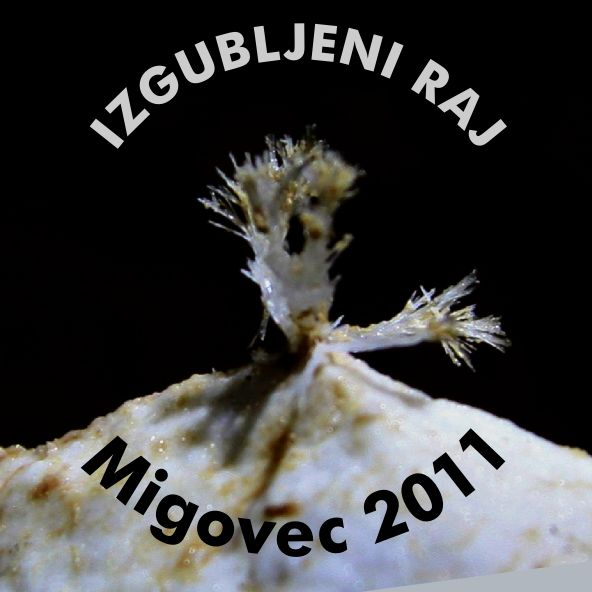
\includegraphics[width=\linewidth]{2011/overview/slov_2011_badge.jpg}} 
 \caption{The 2011 expedition logo. \pen{Jarvist Frost}}
 \label{2011 logo}
\end{marginfigure}

Between 15\textsuperscript{th} July and the 15\textsuperscript{th} August 2011, Imperial College Caving Club
had twenty members participate in the Izgubljeni Raj 2011 expedition to
\passage[mountain]{Tolminski Migovec}, Slovenia. The aims for this expedition were the
continued exploration of \passage{Vrtnarija}, where considerable efforts in
2010 had led to the discovery of 2.2 km of mainly horizontal passage,
all below 500 m in depth. At the start of the expedition,
\passage{Vrtnarija} was 8796 m long and 807 m deep.

This summer we had less manpower than last year, but were still
attempting to set up a similar four-man camp at -550 m (Camp \passage{X-Ray}) and carry out
deep pushing. Our exploration continued routes which were diverse in
direction from camp -- soon we were taking many hours just to travel from
camp to the pushing front and back.

As a result of the reduced manpower and the considerable demands that
exploration of \passage{Vrtnarija} was making on our time, we unfortunately
did not manage to contribute towards the exploration of \passage{Kavkna
Jama} and the attempted connection of the \passage{Migovec} and \passage{Vrtnarija}
systems.

\tweet{9:20PM Jul 15, 2011}{At 4 am as I adjusted tarps in the rain, the words of the great leader,Scuz, came to me;"this is an expedition not a f****ng holiday."Tetley}

Our efforts were considerably hampered by the weather. We had the
wettest summer we've ever experienced on \passage[mountain]{Migovec}. We only very rarely
had sunny enough periods to dry our caving equipment and clothes. A
particularly memorable rainstorm of 48 hours near the beginning of
expedition was rounded off by a heavy snowstorm -- the first we've ever
experienced in 15 summers on this mountain!

\begin{marginfigure}
\checkoddpage \ifoddpage \forcerectofloat \else \forceversofloat \fi
\centering
 \frame{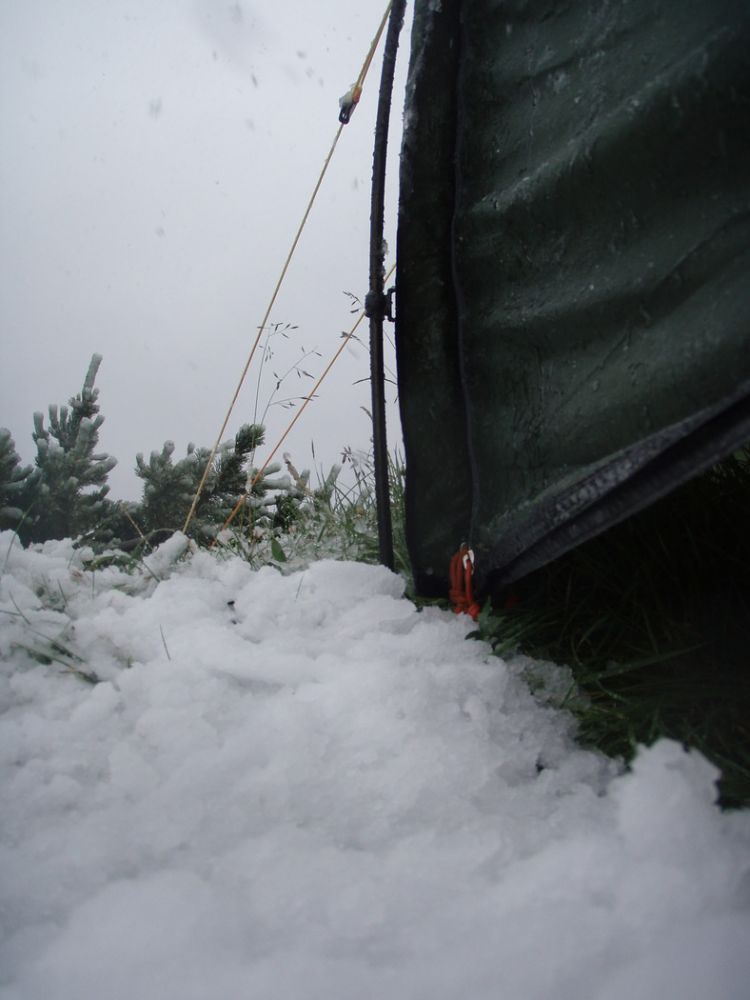
\includegraphics[width=\linewidth]{2011/overview/2011-07-24-08.19.51-Jan Evetts-Olympus Compact-P7240032-Snow Day--orig_1050p.jpg}} 
 \caption{Waking up to snow one morning was unexpected. \pic{Jan Evetts}}
 \label{snow day}
\end{marginfigure}

For two periods of 36 hours, underground camp was effectively cut off
from the surface by high water levels in the cave system, making some of
the pitches impassable. Thanks to the quality, warmth, provisions and
size of underground camp this wasn't a major problem as exploration
simply stopped and the explorers got a lot of sleep instead. Certainly
underground camp was a more pleasant environment than the windswept,
rain lashed and barely above freezing surface of the mountain.

In all we discovered 2229 m of new cave passage taking the cave to 11025
m long and 888 m deep. All these extensions have been made at depths
greater than 500 m, on multi-day trips based at an underground camp.
\passage{Vrtnarija} now has the vast majority of passage, over 8 km, at
depths of greater than 500 m.
